% =============================================================================
% Applied Microeconometrics 2026 - Computer Assignment 1
% Group G3 - Presentation
%
% Compiles with pdfLaTeX.  IMPORTANT: the three figure PDFs must sit in the same
% folder as this file (or in the Overleaf project root):
%     fig1_che_vs_gdp.pdf
%     fig2_trend_by_income.pdf
%     fig3_disease_burden.pdf
%
% SPEAKER NOTES
%   Every frame carries a \note{}. For a PDF with notes pages, uncomment line A.
%   For presenter view on a second screen, uncomment line B. Leave both
%   commented for the version you project.
% =============================================================================
\documentclass[10pt,aspectratio=169,t]{beamer}

% \setbeameroption{show notes}                          % A: slides + notes pages
% \setbeameroption{show notes on second screen=right}   % B: presenter view

\usepackage[T1]{fontenc}
\usepackage{lmodern}
\usepackage{booktabs}
\usepackage{graphicx}
\usepackage{amsmath}
\usepackage{array}

\graphicspath{{./}{figures/}{../output/figures/}}

% --- monochrome theme: black text, no accent colour, no chrome ---------------
\usetheme{default}
\usecolortheme{default}
\setbeamertemplate{navigation symbols}{}
\setbeamertemplate{itemize items}[circle]

\definecolor{g3grey}{RGB}{130,130,130}
\setbeamercolor{structure}{fg=black}
\setbeamercolor{block title}{bg=black!8,fg=black}
\setbeamercolor{block body}{bg=black!3}

% Emphasis is weight, not colour: \alert{...} sets bold black.
\setbeamercolor{alerted text}{fg=black}
\setbeamerfont{alerted text}{series=\bfseries}

% Wider text block than the beamer default, so the tables have room.
\setbeamersize{text margin left=1.6em, text margin right=1.6em}
\setlength{\tabcolsep}{4pt}
\renewcommand{\arraystretch}{1.12}

% Frame title: bold black, no rule underneath.
\setbeamertemplate{frametitle}{%
  \vspace{0.55em}%
  {\large\bfseries\insertframetitle}\par
  \vspace{0.4em}}

% Footline: slide number only.
% To drop the number as well, replace the body below with \hbox{}.
\setbeamercolor{g3foot}{fg=g3grey,bg=}
\setbeamertemplate{footline}{%
  \leavevmode%
  \hbox{\begin{beamercolorbox}[wd=\paperwidth,ht=2.2ex,dp=1.6ex,rightskip=1.6em]{g3foot}%
    \hfill\scriptsize\insertframenumber%
  \end{beamercolorbox}}%
  \vskip0pt}

\setlength{\leftmargini}{1.2em}

\title{\bfseries Determinants of Health Expenditure}
\subtitle{Evidence from a Modern Country-Level Panel}
\author{%
  \normalsize
  \begin{tabular}{@{}l@{\hspace{2em}}l@{}}
    Ashwath Balasubramanian & GE/2025-27/014 \\
    Gyavin Riju             & GE/2025-27/022 \\
    Anirudh R Raman         & GE/2025-27/009 \\
  \end{tabular}}
\institute{\normalsize Group 3}
\date{\footnotesize Applied Microeconometrics 2026 \quad\textbar\quad \today}

\begin{document}

% =============================================================================
\begin{frame}[plain,c]
\titlepage
\vspace{0.5em}
\vfill
{\tiny\color{g3grey}
Reference paper: Xu, K., Saksena, P. and Holly, A. (2011). \textit{The
Determinants of Health Expenditure: A Country-Level Panel Data Analysis.} WHO,
Geneva and Results for Development Institute. \\
Data: World Bank World Development Indicators; WHO Global Health Expenditure
Database.}
\end{frame}

\note{
Thirty seconds. Open with the question, not the paper.

"The question we answer is one of the oldest in health economics. When a country
gets richer, does it spend proportionately more on health? If the income
elasticity is above one, health care is a luxury good and the health share of
GDP rises mechanically with development. If it is below one, health care is a
necessity, and rising health shares need a different explanation."

"We re-estimate this on 145 countries, 2010 to 2021, a window that includes
COVID. Our headline number is 0.744."

Do not read out the names or the roll numbers.
}

% =============================================================================

% =============================================================================
\begin{frame}{(a) Xu, Saksena and Holly (2011)}
\vspace{0.4em}
\begin{block}{Objective}
What drives national health expenditure, and how does it evolve? Written because
the evidence base was almost entirely OECD. Central question: is the income
elasticity above or below one?
\end{block}
\vspace{1em}
\begin{columns}[T]
\begin{column}{0.46\textwidth}
\textbf{Data}
\begin{itemize}\setlength\itemsep{0.4em}
  \item 143 countries, 1995 to 2008
  \item WHO National Health Accounts, SHA 1.0
  \item Disease burden proxied by TB incidence alone
\end{itemize}
\end{column}
\begin{column}{0.50\textwidth}
\textbf{Findings}
\begin{itemize}\setlength\itemsep{0.4em}
  \item Income elasticity \alert{0.75 to 0.95}, below unity
  \item Health care is a \alert{necessity}, not a luxury
  \item No general upward trend in the health share of GDP
\end{itemize}
\end{column}
\end{columns}
\end{frame}

\note{
Forty-five seconds. Three things only.

1. The motivation is coverage. Everything known about the income elasticity came
   from rich countries, and the policy question is about poor ones.
2. Their answer is below one. Health care is a necessity.
3. Flag the TB limitation now, because it sets up the next slide. Say it in
   their words: this was a constraint, not a choice. NCD time series did not
   exist when they wrote.

If asked why they also run Blundell and Bond: GDP and health spending are
jointly determined, so they instrument income with its own lags. We do not,
because the assignment fixes the estimator set to pooled, FE and RE.
}

% =============================================================================
\begin{frame}{(b) How this study differs}
\vspace{0.4em}
\begin{center}
\small
\begin{tabular}{@{}l l l@{}}
\toprule
 & \textbf{Xu et al.\ (2011)} & \textbf{This study} \\
\midrule
Window          & 1995 to 2008, SHA 1.0 & \alert{2010 to 2021}, SHA 2011 \\
Panel           & 143 countries, unbalanced & 145 countries, \alert{balanced}, $N=1740$ \\
Disease burden  & TB incidence only & TB \alert{and NCD mortality} \\
Fiscal capacity & Total government expenditure & Government final consumption \\
Ageing          & Population 60+ & Population 65+ \\
Outcome         & Total, government, out-of-pocket & Total only \\
Estimators      & Pooled, FE, RE, Blundell-Bond & Pooled, FE, RE \\
\bottomrule
\end{tabular}
\end{center}

\vspace{1em}
\begin{itemize}\setlength\itemsep{0.5em}
  \item \textbf{Objective.} Their result rests on a decade of uninterrupted
        growth. We ask whether it survives the largest shock to health spending
        on record.
  \item \textbf{Epidemiological transition.} Burden shifts from infectious to
        chronic as countries grow richer, and NCD burden is itself correlated
        with income, so omitting it biases $\beta_1$.
\end{itemize}
\end{frame}

\note{
One minute. Do not read the table. Let it sit and speak to the two bullets.

The line that matters: "their conclusion was established on a period of
uninterrupted growth. Ours includes 2020. That is the real test."

Be ready for a challenge on fiscal capacity, but do not volunteer it. Answer if
asked: their series, Expense as a per cent of GDP, covers only 76.5 per cent of
our country-years and just 91 of 162 candidate countries across all twelve
years. Government final consumption is narrower, it excludes transfers,
subsidies, interest and capital formation, so it is a lower bound on fiscal
space. We took the complete series because a balanced panel is required for the
tests in part (d) to compare all three models on an identical sample.
}

% =============================================================================
\begin{frame}{(c) The panel}
\vspace{0.4em}
\begin{columns}[T]
\begin{column}{0.47\textwidth}
\textbf{Structure}
\begin{itemize}\setlength\itemsep{0.3em}
  \item $N = 145$ countries, $T = 12$ years
  \item 2010 to 2021, $NT = 1740$
  \item Strictly balanced, and $N \gg T$
\end{itemize}
\vspace{1em}
\textbf{Specification}
\vspace{0.3em}
{\small
\begin{align*}
\ln \mathit{CHE}_{it} = {}& \beta_0 + \beta_1 \ln \mathit{GDP}_{it}
   + \beta_2 \mathit{GFCE}_{it} \\
 & + \beta_3 \mathit{OVER65}_{it} + \beta_4 \ln \mathit{TB}_{it} \\
 & + \beta_5 \mathit{NCD}_{it} + \gamma' \mathit{INC}_i
   + u_i + \varepsilon_{it}
\end{align*}}
\vspace{0.4em}

{\small Log-log, so $\beta_1$ is the income elasticity directly.}
\end{column}
\begin{column}{0.49\textwidth}
\small
\begin{tabular}{@{}lr@{\hspace{1.4em}}lr@{}}
\toprule
\multicolumn{2}{@{}l}{\textbf{Income group}} &
\multicolumn{2}{l@{}}{\textbf{Region}} \\
\cmidrule(r){1-2}\cmidrule(l){3-4}
High         & 52 & Europe and Central Asia  & 47 \\
Upper middle & 42 & Sub-Saharan Africa       & 37 \\
Lower middle & 36 & Latin America and Carib. & 20 \\
Low          & 15 & Middle East and N.\ Afr. & 18 \\
             &    & East Asia and Pacific    & 17 \\
             &    & South Asia               &  4 \\
             &    & North America            &  2 \\
\midrule
Total & 145 & Total & 145 \\
\bottomrule
\end{tabular}
\end{column}
\end{columns}
\end{frame}

\note{
Thirty seconds. Two points, then move.

"Balanced. That matters because all three estimators must run on an identical
sample for the tests in part (d) to be valid comparisons."

"Log-log in expenditure and income, so beta one is the elasticity itself, and
research question one reduces to testing beta one equals one. Percentage
variables, government consumption, the over-65 share and NCD mortality, enter in
levels, so their coefficients read as the effect of a one percentage point
change."

Do not walk through the region table. It is there to show the coverage is not
OECD-only, which was the whole motivation of the reference paper.
}

% =============================================================================
\begin{frame}{(c) Expenditure against income}
\begin{columns}[c]
\begin{column}{0.55\textwidth}
\begin{center}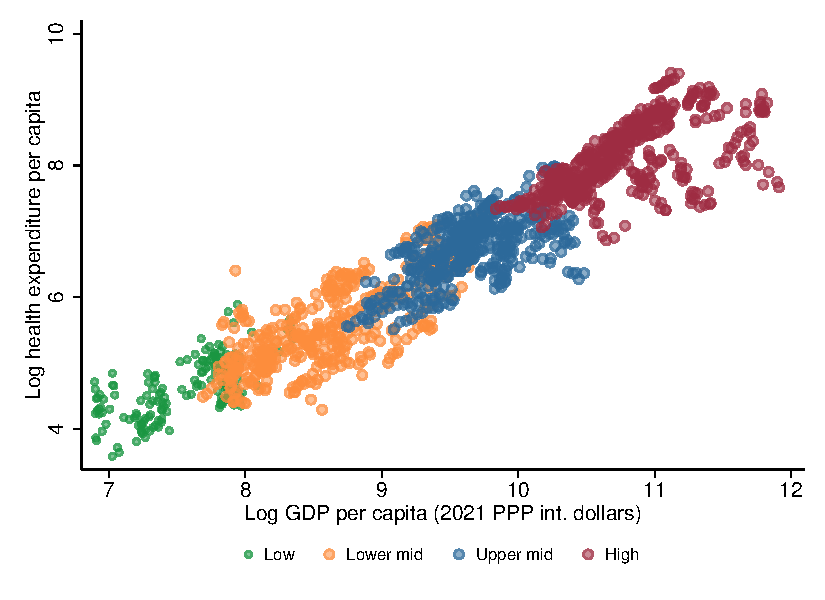
\includegraphics[height=0.68\textheight]{fig1_che_vs_gdp}\end{center}
\end{column}
\begin{column}{0.43\textwidth}
\begin{itemize}\setlength\itemsep{0.9em}
  \item Strong, tight, close to \alert{linear in logs}.
  \item Income groups form ordered, overlapping bands.
  \item The high income band \alert{fans out}: same income, very different
        spending.
  \item That dispersion is the unobserved heterogeneity motivating fixed
        effects.
\end{itemize}
\end{column}
\end{columns}
\end{frame}

\note{
Forty seconds. This slide does one job: it sets up fixed effects visually.

Point at the right-hand side of the cloud. "Two countries here have the same GDP
per capita and spend a factor of two apart on health. Whatever explains that is
not in our regressor list. It is health system design, relative medical prices,
institutional quality. It is time-invariant and it is correlated with income.
That is exactly what u-i is, and it is why we end up rejecting pooled OLS."
}

% =============================================================================
\begin{frame}{(c) The health share of GDP over time}
\begin{columns}[c]
\begin{column}{0.55\textwidth}
\begin{center}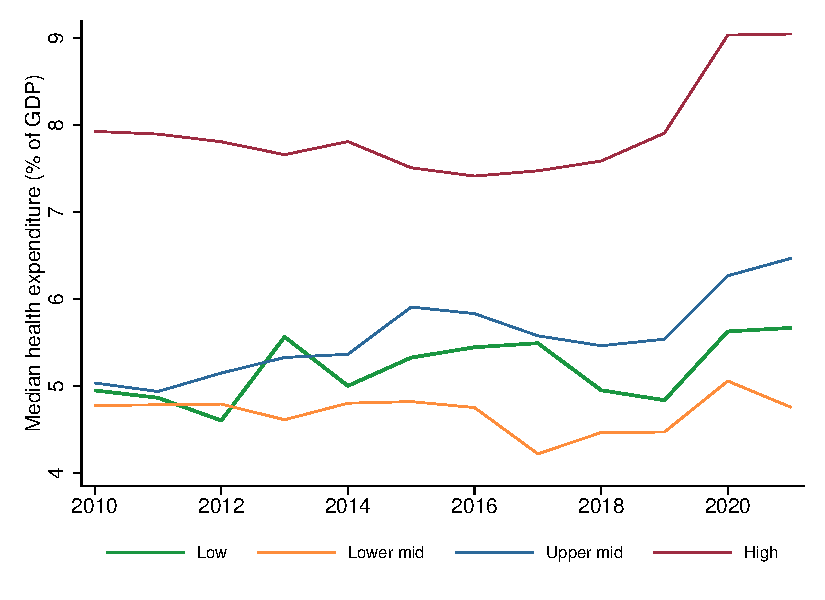
\includegraphics[height=0.68\textheight]{fig2_trend_by_income}\end{center}
\end{column}
\begin{column}{0.43\textwidth}
\begin{itemize}\setlength\itemsep{0.9em}
  \item The income gradient is \alert{stable} throughout.
  \item No group trends through 2019, reproducing Xu et al.
  \item \alert{2020 breaks every series}: the high income median moves 7.9 to
        9.0 per cent of GDP.
  \item Common, not outlier-driven: 127 of 145 countries rise.
\end{itemize}
\end{column}
\end{columns}
\end{frame}

\note{
Forty seconds. This is the slide that justifies time dummies.

"Two readings. First, the pre-2019 flatness is Xu et al.'s result reappearing on
a completely different window and a different accounting basis. That is
reassuring for replication."

"Second, 2020 is a level shift that hits every income group at once. It is a
common time effect. If we leave year dummies out, that shock loads onto whatever
regressor happens to be trending, and in part (e) we will see it do exactly
that."

Numbers if asked: high income runs 7.4 to 7.9 per cent through 2019, the other
three groups 4.2 to 6.5.
}

% =============================================================================
\begin{frame}{(c) Disease burden across the income gradient}
\begin{center}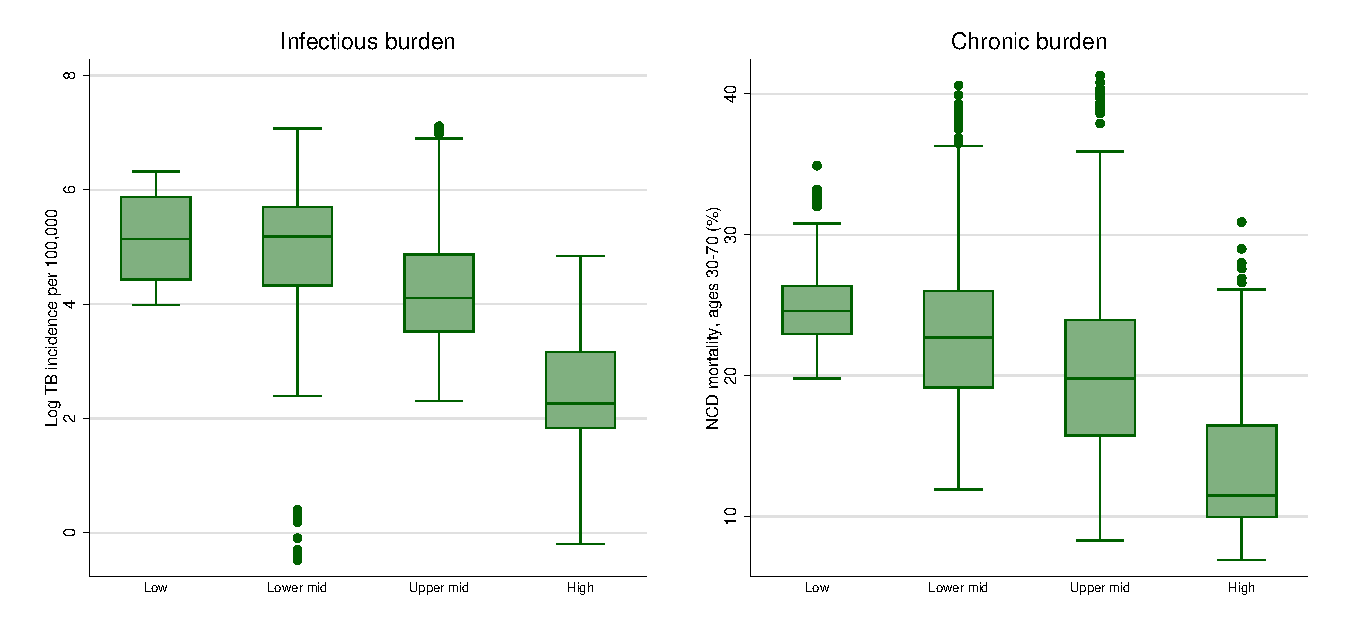
\includegraphics[height=0.46\textheight]{fig3_disease_burden}\end{center}
\vspace{0.8em}
\begin{itemize}\setlength\itemsep{0.45em}
  \item TB falls eighteen-fold across the gradient, median 172 per 100,000 to
        10. \alert{The left panel is on a log scale.}
  \item NCD mortality only halves, 24.6 to 11.5 per cent.
  \item TB alone would understate disease burden precisely where health spending
        is highest.
\end{itemize}
\end{frame}

\note{
Thirty seconds. This slide justifies our one substantive addition to the paper.

Say the log-scale caveat before anyone raises it: "the left panel is
logarithmic, so its gradient is much steeper than it looks sitting next to the
right panel."

The punchline: "TB alone is a good proxy for disease burden in poor countries
and a bad one in rich countries. Since income is our regressor of interest, a
proxy whose quality varies systematically with income is the worst kind of
measurement error to have."
}

% =============================================================================
\begin{frame}{(c) Summary statistics: \texttt{xtsum}}
\vspace{0.3em}
\begin{center}
\scriptsize
\setlength{\tabcolsep}{6pt}
\renewcommand{\arraystretch}{0.92}
\begin{tabular}{@{}ll rrrr l@{}}
\toprule
Variable & & Mean & Std.\ dev. & Min & Max & Obs. \\
\midrule
Log health expenditure p.c. & overall & 6.743 & 1.355 & 3.582 & 9.408 & $N=1740$ \\
 & between & & 1.349 & 3.886 & 9.266 & $n=145$ \\
 & within  & & \alert{0.162} & 5.870 & 7.443 & $T=12$ \\
\addlinespace
Log GDP per capita & overall & 9.585 & 1.153 & 6.896 & 11.912 & $N=1740$ \\
 & between & & 1.153 & 6.923 & 11.786 & $n=145$ \\
 & within  & & \alert{0.096} & 9.176 & 9.988 & $T=12$ \\
\addlinespace
Govt final consumption (\% of GDP) & overall & 16.756 & 7.138 & 2.360 & 103.164 & $N=1740$ \\
 & between & & 6.714 & 5.584 & 62.615 & $n=145$ \\
 & within  & & \alert{2.483} & $-$17.664 & 57.305 & $T=12$ \\
\addlinespace
Population aged 65+ (\% of total) & overall & 8.884 & 6.392 & 0.862 & 29.217 & $N=1740$ \\
 & between & & 6.361 & 1.091 & 26.702 & $n=145$ \\
 & within  & & \alert{0.806} & 5.280 & 12.138 & $T=12$ \\
\addlinespace
Log TB incidence & overall & 3.876 & 1.501 & $-$0.478 & 7.115 & $N=1740$ \\
 & between & & 1.489 & 0.052 & 6.746 & $n=145$ \\
 & within  & & \alert{0.220} & 2.966 & 4.799 & $T=12$ \\
\addlinespace
NCD mortality, ages 30--70 (\%) & overall & 19.007 & 6.917 & 6.900 & 41.300 & $N=1740$ \\
 & between & & 6.835 & 8.508 & 39.617 & $n=145$ \\
 & within  & & \alert{1.189} & 11.932 & 25.224 & $T=12$ \\
\bottomrule
\end{tabular}
\end{center}
\vspace{0.3em}

\end{frame}

\note{
One minute. This is the raw output AND the interpretation, since the ratio
slide is gone. Read it, do not just show it.

Say what the three rows are, once: "overall is every country-year pooled
together. Between is the 145 country averages. Within is how much one country
moves around its own average."

Then the number that matters, pointing at log GDP: "between standard deviation
1.153, within standard deviation 0.096. A ratio of twelve. Two randomly chosen
countries differ in income about twelve times more than one country differs
between two randomly chosen years. In variance terms only 0.7 per cent of the
variation in income is within-country."

Then the payoff, said explicitly so part (e) is not a surprise:
"Fixed effects throws the between variation away, so for income it works with
0.7 per cent of the variance. Expect a much larger FE standard error on income,
and expect the slow-moving variables, ageing and NCD mortality, to fall apart
under FE once year dummies take out the common trend. Both things happen."

The exception, worth naming: "government final consumption is the one regressor
with real within-country movement, 12 per cent of its variance. It is the only
one significant in every column of the next table, and that is not a
coincidence."

Income group is not in this table because it has nothing to decompose: its
within standard deviation is exactly zero, so fixed effects cannot identify it
at all. Say that when the FE column comes up blank on the results slide. Be
precise about why it is zero: the World Bank reclassifies economies every year
and several countries did move group between 2010 and 2021, but the API serves
one current classification per country with no year dimension, and we apply it
to all twelve years. Time-invariant by construction, not because the world stood
still. If challenged: the assignment requires a time-invariant regressor, the
historical OGHIST series is not on the API, and the cost is that a country
reclassified mid-window carries its end-of-period status throughout.

Two facts held in reserve:
- The negative within minimum for government consumption is not a negative
  share. xtsum adds the grand mean back, so a within value of minus 17.7 means a
  country running 34 points below its own average. Both extremes are Timor-Leste,
  at 103 per cent of GDP in 2010 and 28 per cent by 2021.
- Bangladesh has zero within variation in TB, a constant 221 per 100,000 for all
  twelve years, so it contributes nothing to the FE TB coefficient.
}

% =============================================================================
\begin{frame}{(d) Tests of hypotheses, and the estimated $\lambda$}
\vspace{0.4em}
\begin{center}
\footnotesize
\setlength{\tabcolsep}{5pt}
\begin{tabular}{@{}l l c c c@{}}
\toprule
\textbf{Comparison} & \textbf{$H_0$} & \textbf{No time dummies}
& \textbf{With time dummies} & \textbf{Decision} \\
\midrule
(i) Pooled vs FE, F test & $u_i = 0$ for all $i$
   & $F(144,1590) = 55.80$ & $F(144,1579) = 59.71$ & Reject $H_0$ \\
(ii) Pooled vs RE, BP LM & $\mathrm{Var}(u_i) = 0$
   & $LM = 6302.74$ & $LM = 6358.42$ & Reject $H_0$ \\
(iii) FE vs RE, Hausman & $\mathrm{Cov}(u_i, X_{it}) = 0$
   & $\chi^2(5) = 20.84$ & $\chi^2(5) = 78.04$ & Reject $H_0$ \\
\bottomrule
\end{tabular}
\end{center}
\vspace{0.2em}
{\scriptsize $p < 0.001$ throughout, except (iii) without time dummies, where
$p = 0.001$.}

\vspace{0.9em}
\begin{block}{Random effects: the estimated $\lambda$}
\vspace{0.2em}
\centering
$\hat\lambda \;=\; 1 - \sqrt{\dfrac{\hat\sigma^2_\varepsilon}
{T\hat\sigma^2_u + \hat\sigma^2_\varepsilon}} \;=\; \mathbf{0.872}$

\vspace{0.4em}
{\footnotesize $\hat\sigma_u = 0.275$, \quad
$\hat\sigma_\varepsilon = 0.123$, \quad $\rho = 0.834$, \quad $T = 12$, \quad
$\hat\lambda = 0.868$ without time dummies}
\end{block}
\end{frame}

\note{
Ninety seconds. Take the three tests fast, then spend the time on lambda.

(i) "F test on the joint significance of the 144 country effects, read off the
foot of xtreg fe. Rejects. Country effects exist."

(ii) "Breusch and Pagan LM. Null is that the variance of u-i is zero. Rejects.
Same verdict from the random effects side. Note the distribution is chi-bar
squared, a fifty-fifty mixture, because the null puts a variance on the boundary
of the parameter space."

(iii) "Hausman. Null is that u-i is uncorrelated with the regressors, so RE is
consistent and efficient. Rejects at 0.1 per cent."

Then lambda, slowly, because this is what the question specifically asks for:

"Lambda is the quasi-demeaning weight. Random effects does not use raw data and
it does not use fully demeaned data. It subtracts lambda times the country mean.
At zero you get pooled OLS, at one you get fixed effects. Ours is 0.872."

"Lambda is high because rho is 0.834: five-sixths of the residual variance is
the country effect. With T equal to twelve and country effects that strong, GLS
leans hard on within variation."

Do NOT say a high lambda means RE is nearly FE. Quasi-demeaning at 0.872 shrinks
the between-country standard deviation of log GDP from 1.153 to 0.147, but the
within standard deviation is only 0.096. So the regressor RE actually runs on is
still 70 per cent between-country variation. Lambda describes the
transformation, not where the estimate lands.

Then give the verdict out loud, since no slide now carries it:
"All three reject. Pooled OLS is out on two independent tests, and Hausman puts
random effects out as well. The preferred specification is fixed effects with
time dummies."

Add the honesty line, which is the one that earns marks: "the Hausman test
rejects on the joint coefficient vector. Our parameter of interest moves only
from 0.746 under RE to 0.744 under FE, against a standard error near 0.10. So
the model choice is defensible, but it is not what drives our headline number."

Two honest caveats, if asked:
- All three tests use conventional standard errors, because none of them is
  reported under vce(cluster). Hausman in particular needs RE to be efficient
  under the null, which clustering breaks.
- Income group is dropped from the Hausman test: FE cannot identify a
  time-invariant regressor and the test needs a shared coefficient vector. With
  time dummies Stata reports the differenced covariance matrix is rank 5 against
  16 coefficients and not positive definite, so we treat 78.04 as corroborating
  and lean on the clean 20.84. Both reject.

Held in reserve, an argument that needs no test: 145 countries with complete
data are closer to the population than to a random draw from it. Random effects
treats each country effect as a draw from a distribution; we are not sampling
countries, we have nearly all of them. Each effect is better treated as a
separate intercept, which is mechanically what FE does. Wooldridge makes this
point for policy analysis on aggregated data, page 493. We still report RE,
because FE cannot identify income group at all.
}

% =============================================================================
\begin{frame}{(e) Pooled OLS, fixed effects and random effects}
\vspace{0.2em}
\begin{center}
\scriptsize
\setlength{\tabcolsep}{4.6pt}
\renewcommand{\arraystretch}{0.88}
\begin{tabular}{@{}l cccccc@{}}
\toprule
& \multicolumn{3}{c}{\textbf{Without time dummies}} & \multicolumn{3}{c}{\textbf{With time dummies}} \\
\cmidrule(lr){2-4}\cmidrule(lr){5-7}
Dependent variable: $\ln \mathit{CHE}_{it}$ & Pooled & FE & RE & Pooled & \textbf{FE} & RE \\
\midrule
Log GDP per capita      & 0.798*** & 0.773*** & 0.761*** & 0.800*** & \alert{0.744***} & 0.746*** \\
                        & (0.062) & (0.096) & (0.075) & (0.063) & \alert{(0.102)} & (0.085) \\
Govt final consumption  & 0.014*** & 0.020** & 0.019** & 0.014*** & 0.017** & 0.017** \\
                        & (0.004) & (0.008) & (0.007) & (0.004) & (0.007) & (0.007) \\
Population 65+          & 0.041*** & 0.023** & 0.030*** & 0.041*** & $-$0.000 & 0.021*** \\
                        & (0.004) & (0.009) & (0.005) & (0.004) & (0.012) & (0.006) \\
Log TB incidence        & $-$0.090*** & $-$0.074* & $-$0.075*** & $-$0.089*** & 0.002 & $-$0.041* \\
                        & (0.027) & (0.040) & (0.028) & (0.028) & (0.031) & (0.023) \\
NCD mortality           & $-$0.013*** & $-$0.014** & $-$0.013*** & $-$0.013*** & $-$0.007 & $-$0.010* \\
                        & (0.004) & (0.006) & (0.005) & (0.004) & (0.006) & (0.005) \\
\addlinespace[2pt]
Lower middle income     & $-$0.020 & -- & 0.029 & $-$0.021 & -- & 0.075 \\
                        & (0.106) & & (0.106) & (0.107) & & (0.115) \\
Upper middle income     & 0.082 & -- & 0.223 & 0.080 & -- & 0.353* \\
                        & (0.148) & & (0.151) & (0.150) & & (0.188) \\
High income             & 0.035 & -- & 0.307 & 0.033 & -- & 0.604** \\
                        & (0.195) & & (0.196) & (0.201) & & (0.280) \\
\midrule
Observations / countries & 1740 & 1740 / 145 & 1740 / 145 & 1740 & 1740 / 145 & 1740 / 145 \\
$R^2$                    & 0.953 & 0.445 & 0.444 & 0.953 & 0.481 & 0.473 \\
$\lambda$                & & & 0.868 & & & \alert{0.872} \\
\bottomrule
\end{tabular}
\end{center}
\vspace{0.2em}
{\scriptsize Cluster-robust standard errors by country in parentheses.
*** $p<0.01$, ** $p<0.05$, * $p<0.10$.}
\end{frame}

\note{
Two and a quarter minutes. This slide now carries the whole cross-model
comparison, so do not rush it. Orient first, then robust, then fragile.

ORIENT (20 seconds). "Six columns. Three estimators, first without time dummies
and then with. Cluster-robust standard errors by country throughout. Column
five, fixed effects with time dummies, is our preferred specification, and 0.744
is the number the whole study turns on."

Two structural features, then stop describing:
- The FE columns are blank for income group. Fixed effects absorbs anything
  time-invariant, and our income classification has a within standard deviation
  of exactly zero. Not a missing result, the estimator working as designed.
- Year dummies are jointly significant in all three models: F of 4.29 pooled,
  6.51 under FE, chi-squared of 58.56 under RE. Common time effects belong in
  the specification, which vindicates the 2020 break on the trend figure.

WHAT IS ROBUST (45 seconds). Point along the top row.
"Income. Six columns, six times significant at one per cent, six times below
one, range 0.744 to 0.800. Sign, significance and magnitude are all stable.
Whatever you believe about country effects, you get the same answer."

Then the price of FE, pointing at the standard errors: "0.062 pooled against
0.102 under FE, a 65 per cent increase on identical data. Fixed effects is not
free. It buys consistency by discarding 99 per cent of the variation in the
regressor, and you pay in precision."

Then government consumption: "the only regressor significant in every single
column, 0.014 to 0.020, and not a coincidence: it is the only one with real
within-country variation, twelve per cent. A one percentage point rise in the
government consumption share goes with 1.4 to 2.0 per cent higher health
spending per capita. Fiscal capacity is the robust time-varying driver here."

WHAT IS FRAGILE (60 seconds). Point down the FE columns.
"Now the three that move. Without year dummies, ageing enters at 0.023 and log
TB at minus 0.074, both significant. Add year dummies and ageing goes to
essentially zero, TB to 0.002, NCD loses significance. Pooled, by contrast,
moves in the third decimal."

State the mechanism carefully, because the obvious explanation is wrong: "it is
not that no variation is left. Year dummies remove about half the within-country
variation in ageing and TB, and a third in NCD mortality. Two thirds survives.
What year dummies take is the part every country shares. Every country is
ageing, every country's TB is falling, at the same time that health spending is
rising everywhere. Without year effects, fixed effects credits that common drift
to whichever regressor drifts alongside it."

The contrast that proves it: "government consumption loses only three per cent
of its within variation to year dummies, because fiscal shares move on each
country's own political schedule. That is the one regressor whose variation is
genuinely country-specific, and it is the one that survives everywhere."

So the honest conclusion is not that ageing does not matter for health
expenditure. It is that twelve years of within-country variation, net of a
common trend, cannot identify it.

RE VERSUS FE (20 seconds). "Random effects sits at 0.746, right beside fixed
effects at 0.744. Lambda is 0.872, but that is not the reason: after
quasi-demeaning the regressor is still 70 per cent between-country. What strips
the between identification is the income dummies, which explain 87 per cent of
the cross-country variation in log GDP. Replace them with region dummies and RE
returns to 0.818, while FE stays at 0.744 whatever control we use."

Income group is the one real disagreement: FE absorbs it, pooled finds it
insignificant because log GDP already carries the income gradient, and RE
recovers a high income premium of 0.604. Treat that premium with caution: it is
identified purely off between-country variation, which Hausman tells us not to
trust, and the classification itself is measured from 2025 GNI.

If anyone asks about the 0.953 R-squared: not comparable with the 0.445. The
first is overall fit dominated by between-country variation, the second is
within-country fit. Different quantities.
}

% =============================================================================
\begin{frame}{(e) Interpreting the income coefficient}
\vspace{0.5em}
\begin{block}{The income elasticity: $\hat\beta_1 = 0.744$, s.e.\ $0.102$}
A one per cent rise in real GDP per capita \emph{within} a country is associated
with a \alert{0.744 per cent} rise in real health expenditure per capita,
holding fiscal capacity, ageing, disease burden and common year effects
constant.
\end{block}

\vspace{1em}
\begin{itemize}\setlength\itemsep{0.75em}
  \item Because the specification is log-log, this \textbf{is} the income
        elasticity. Research question 1 reduces to a single test.
  \item \textbf{$H_0 : \beta_1 = 1$ gives $F(1,144) = 6.29$, $p = 0.013$.}
        Rejected at 5 per cent: health expenditure grows \alert{more slowly}
        than income.
  \item \textbf{Health care is a necessity, not a luxury.} Growth alone predicts
        a \emph{falling} health share of GDP. Rising shares need another
        explanation: technology, relative prices, ageing, policy.
  \item \textbf{Xu et al.\ survive re-estimation.} 0.744 sits at the lower edge
        of their 0.75 to 0.95 range, on a different decade and a window
        containing COVID.
\end{itemize}
\end{frame}

\note{
Ninety seconds. This is the core of the talk. Slow down here.

Give the interpretation in one clean sentence and stress the word "within":
"this is not rich countries spend more than poor countries. It is the same
country spending more as it grows. That distinction is the entire reason we are
using panel data rather than a cross-section."

Then the test. "Because it is log-log the coefficient is the elasticity, so the
luxury-versus-necessity question is just a test of whether it equals one. F of
6.29, p of 0.013. Rejected. Below one. Necessity."

Then the economics, which is what earns the marks: "the policy implication is
that you cannot explain rising health shares of GDP by saying countries got
richer. Growth alone predicts a falling share. So the rise has to come from
somewhere else: medical technology, relative price growth in a labour-intensive
sector, ageing, or deliberate policy expansion."

Close on replication: "we changed the decade, the accounting standard, the
fiscal variable and the age cutoff, we added NCD burden, and we included a
pandemic. The elasticity barely moved. That is a genuinely robust finding."

Two answers to hold ready:
- Does 0.744 differ from their 0.75? No. It is within a tenth of a standard
  error. We are not claiming a lower elasticity, we are claiming the same one.
- Is it causal? No, and say so before being asked. It is a conditional
  within-country association. Health spending is a component of GDP, so income
  is not strictly exogenous. That is the first item on the extensions slide.
}

% =============================================================================
\begin{frame}{(f) Conclusions, and what we would do next}
\vspace{0.4em}
{\small
\begin{columns}[T]

\begin{column}{0.47\textwidth}
\textbf{What we found}
\vspace{0.4em}
\begin{enumerate}\setlength\itemsep{0.55em}
  \item \textbf{FE with time dummies is preferred.} Pooled OLS is rejected by
        the F and LM tests; RE by Hausman.
  \item \textbf{The income elasticity is 0.744, below one.} Health care is a
        necessity: growth alone predicts a \emph{falling} health share of GDP.
  \item \textbf{Xu et al.\ survive re-estimation} on a modern window, a revised
        accounting basis, an added NCD regressor and the COVID shock.
\end{enumerate}
\end{column}

\begin{column}{0.47\textwidth}
\textbf{What we would do next}
\vspace{0.4em}
\begin{enumerate}\setlength\itemsep{0.55em}
  \item \textbf{Address simultaneity.} Health spending is part of GDP, so income
        is not strictly exogenous. Use earlier income in its place.
  \item \textbf{Widen and sharpen the regressors.} Income group is fixed at one
        current classification; a year-by-year series would be better.
  \item \textbf{Go beyond total spending.} Split into government-funded and
        out-of-pocket to show \emph{who} pays as a country gets richer.
\end{enumerate}
\end{column}

\end{columns}}
\end{frame}

\note{
Ninety seconds for the whole slide. Findings fast, extensions slower.

FINDINGS (35 seconds). Three points, roughly one breath each. Do not elaborate;
the elaboration already happened in part (e).

The sentence to land on is the second: "growth alone predicts a falling health
share." It is counter-intuitive, it is the paper's actual contribution, and it
is what an audience remembers.

EXTENSIONS (55 seconds). This is where an examiner will probe. Lead with the
first, because it is the real weakness and volunteering it beats being caught.

Say it in plain words, no jargon needed:
"Our number says health spending and income move together within a country. It
does not prove that growth caused the spending, and the reason is almost silly:
health spending is counted inside GDP. So the thing we are explaining sits
inside the thing we are explaining it with. The standard fix is to use the
country's income from earlier years, because the past cannot be caused by today.
That is what Xu et al. do. We could not, because the assignment fixes us to
pooled, FE and RE."

On the second, own the income group limitation rather than waiting to be asked:
"the World Bank reclassifies countries every year, but the API gives one current
classification per country with no year dimension, so ours is time-invariant by
construction. A country reclassified mid-window carries its end-of-period status
throughout. It matters more than it looks, because the classification explains
87 per cent of the cross-country variation in log GDP."

Do not go deeper unless they push. If they do, the names are Blundell-Bond for
the first point and OGHIST, the World Bank's historical classification
spreadsheet, for the second.

Two answers held in reserve, no longer on the slide:
- If asked whether 2020 breaks the standard errors: yes. Cluster-robust errors
  assume countries are independent, and a pandemic hits all 145 at once.
  Driscoll-Kraay standard errors allow a shared worldwide shock.
- If asked how you could keep income group without giving up FE: a Mundlak
  correction. In practice you just add each country's average income as an extra
  regressor in the RE model. You get the FE answer on the time-varying variables
  and still get a coefficient on income group. Hausman-Taylor does the same job.

Stop here. Thank them and take questions.
}

% =============================================================================
\begin{frame}[plain,c]
\begin{center}
{\Large\bfseries Thank you.}
\end{center}
\end{frame}

\note{
Leave this up through the Q and A.

Likely questions, with short answers:

Q. Why not cluster-robust standard errors for the tests in part (d)?
A. Those tests rely on the classical variance structure. Hausman in particular
   needs RE to be efficient under the null, which clustering breaks. We cluster
   for the coefficient tables, which is where it matters.

Q. Why is lambda so high?
A. T is twelve and rho is 0.834. Five-sixths of the residual variance is the
   country effect, so GLS weights within variation heavily.

Q. Why include the income dummies at all, if FE cannot identify them?
A. Two reasons. They are the assignment's required time-invariant regressor, and
   they are identified in pooled OLS and RE, which is where the high income
   premium of 0.604 comes from. FE absorbing them is itself a result worth
   showing.

Q. Did no country really change income group in twelve years?
A. Countries did; our variable does not. The World Bank API serves one current
   classification per economy with no year dimension, so we apply it to all
   twelve years. The historical series is the OGHIST spreadsheet, which the API
   does not expose. The cost is that a country reclassified mid-window carries
   its end-of-period status throughout.

Q. Why is the TB coefficient negative?
A. Not a demand response. Conditional on income, TB incidence marks weak health
   systems and residual underdevelopment.

Q. An R-squared of 0.953 for pooled OLS?
A. Overall fit, dominated by between-country variation. Not comparable with the
   0.445 within figure for FE.

Q. Why a balanced panel? Are you not throwing away countries?
A. Yes, and deliberately. The three tests in part (d) are only valid comparisons
   if all three estimators run on an identical sample.

Q. Why 2010 as the start?
A. SHA 2011 coverage. Earlier years are on the old accounting basis and are not
   comparable. The window ends in 2021 because that is the last year NCD
   mortality is published.
}

\end{document}
